\chapter{Transports collectifs}

% \textit{Mobilité pour Tous : les transports collectifs comme pilon
%   central de la mobilité métropolitaine}

Si le vélo et la marche sont des moyens de transport économiques et
adaptés à environ la moitié de la population pour de courts trajets de
quelques kilomètres, une autre partie de la population nécessite une
alternative. Que ce soit en raison de l'absence de vélo, de problèmes
de santé, de la préférence pour d'autres modes de transport ou de la
nécessité de parcourir de plus longues distances, tous n'opteront pas
pour la marche ou le vélo. En effet, si la majorité des déplacements
au sein de la Métropole sont courts, la plupart des trajets qui
touchent la métropole dépassent ses frontières et sont plus longs.

Historiquement, nous avons considéré les transports en commun
principalement comme un moyen d'accéder au travail en France, limitant
ainsi leur pertinence en dehors des heures de pointe. Cette
perspective a renforcé l'idée que la voiture reste essentielle pour la
majorité des déplacements.

Percevoir la Métropole et la région comme des vecteurs de mobilité
nous conduit inévitablement à envisager les transports collectifs
comme un service uniformément disponible tout au long de la journée et
de la soirée. Votre voiture part lorsque vous le décidez. Si les
transports en commun ne répondent pas à cette simple exigence, ils ne
pourront jamais prétendre à leur juste place comme une option parmi
d'autres.

Pour que les transports collectifs deviennent véritablement une
solution de mobilité fiable et complète, la refonte de notre approche
est nécessaire pour assurer la disponibilité et l'efficacité des
transports collectifs à tout moment de la journée.


\section{Transitions fluides entre systèmes}

% \textit{Harmonisation des Règles et Réglementations des Transports
%   Publics : Vers une Mobilité Sans Frontières}

Lors de nos déplacements en voiture, nous sommes habitués à
reconnaître les panneaux de signalisation et les règles routières au
fur et à mesure de notre trajet, à emprunter les routes de notre
choix, à faire le plein (essence ou électricité) sans se soucier du
fournisseur, et même à traverser les frontières communales et
nationales en toute simplicité.

Cependant, lorsque nous optons pour les transports en commun, les
règles changent d'une commune à l'autre, d'une région à l’autre. Le
tarif (avec toutes ses complexités locales) doit être payé séparément
et à l'aide d'un instrument différent à chaque fois. Même la
navigation exige souvent l'utilisation d'un nouvel outil à chaque
changement de contrôle administratif.

Afin de permettre aux citoyens de voyager comme bon leur semble, avec
un seul tarif et un unique moyen de paiement, il est impératif que les
agglomérations et les régions collaborent pour harmoniser les règles
et les réglementations entre les différents systèmes de transport
public (incluant les bus, les cars, les trains, les bateaux et les
locations de vélos). Nous devons rapidement évoluer vers un système
similaire à celui des Pays-Bas, de Londres et de Lisbonne (pour citer
trois exemples), qui autorise les utilisateurs même non enregistrés à
voyager en utilisant les instruments de paiement sans contact (carte
bancaire, téléphone) qu'ils possèdent déjà, sans inscription au
préalable.

Cette transition vers un système intégré au niveau des règles
tarifaires et instruments de paiement permettra d'offrir aux usagers
une expérience de déplacement fluide, prévisible et cohérente, tout en
simplifiant les démarches administratives et les modes de paiement.

\refs

\link{https://www.intelligenttransport.com/transport-articles/73782/mobile-ticketing-contactless-payment-germany/}

\link{https://tfl.gov.uk/fares/how-to-pay-and-where-to-buy-tickets-and-oyster/pay-as-you-go/contactless-and-mobile-pay-as-you-go}


\section{Une fréquence crédible}

Les transports collectifs des agglomérations jouent un rôle clé grâce
à la fréquence des passages, à la portée de leur service et à la
cohérence du maillage entre les différentes lignes. Toutefois, pour
certaines lignes, la fréquence de passage est si faible qu'elle
compromet l'efficacité du maillage. De ce fait, l'attrait de ces
lignes se limite aux utilisateurs les plus patients.

Actuellement, de nombreux déplacements matinaux et vespéraux sont
effectués en voiture, principalement parce que les correspondances
entre les différents modes de transport ne sont pas optimisées pour le
confort des voyageurs.

Pour assurer une mobilité fluide et une prévisibilité des trajets, il
est essentiel de garantir une fréquence de passage régulière sur
l'ensemble des lignes tout au long de leur période d'opération.


\section{Redynamiser le TER pour une mobilité crédible}

La mobilité est l'épine dorsale de toute région, toute métropole en
plein essor : les Pays de la Loire, avec Nantes Métropole en son cœur,
n'est pas une exception. Le transport régional (TER et car Aléop) a un
rôle crucial à jouer pour assurer une mobilité durable et efficiente
pour tous. Cependant, à l'heure actuelle, ni le TER ni le car n'est
considéré comme une option de mobilité crédible pour de nombreux
citoyens.

L'un des principaux défis est sa fréquence insuffisante. Pour attirer
plus d'usagers et répondre aux besoins de mobilité croissants, il est
impératif d'augmenter la fréquence des trains. Une plus grande
fréquence réduit les temps d'attente, rendant le voyage en train plus
attrayant par rapport à d'autres modes de transport moins écologiques.

La prévisibilité est la clé de la confiance. Si les citoyens savent
qu'un train passe toutes les 15 minutes, par exemple, ils n'ont pas
besoin de consulter constamment un horaire. Cela leur permet de se
rendre à la gare avec l'assurance qu'ils n'attendront pas
longtemps. Un intervalle uniforme et prévisible, tout au long de la
journée, renforce la crédibilité du TER et du car comme moyen de
transport fiable, réduisant ainsi la nécessité du recours à la
voiture.

Une véritable option de transport doit être disponible lorsque les
gens en ont besoin. Le TER et le car doivent fonctionner tôt le matin
pour ceux qui commencent leur journée avant l'aube et continuer tard
le soir pour ceux qui rentrent après une longue journée ou une sortie
vespérale. En élargissant l'amplitude des heures de fonctionnement,
nous assurons que le train est une option de mobilité viable et
crédible, quel que soit le moment de la journée.

Un objectif minimal doit être un cadencement toutes les 15 minutes
toute la journée à l'exception des petites heures de la nuit.


\section{De nouvelles lignes}

Au cours de ces cinquante dernières années, nous avons progressivement
abandonné les lignes de train régionales en France. Un réseau jadis
bien connecté s'est réduit au point que nous évoquons l'expression «
étoile ferroviaire » à Nantes sans percevoir l'ironie qu'elle
renferme, car il ne reste en réalité que cela.

Le rail constitue l'épine dorsale idéale d'un système de transport
public.

Il est impératif de rouvrir les lignes ferroviaires là où cela reste
possible. Plusieurs exemples se présentent, tels que l'Île de Nantes
(la
\href{https://www.mobilitains.fr/tb/t/ligne-johanna-rolland-2021/}{Ligne
  Johanna Rolland}) et les lignes en direction du Pellerin, de
Paimbœuf, de Grand Lieu et de Carquefou, ainsi que la ligne
Saint-Nazaire - Redon.

Deuxièmement, il nous faut examiner où de nouvelles lignes ou des
lignes renforcées seraient pertinentes. Nombre de nos lignes ne
comportent qu'une voie unique sans possibilité de dépassement. Le jour
où nous souhaiterons augmenter le service, nous serions confrontés à
un délai de 15 ans en raison du simple besoin de construire des zones
de dépassement et des systèmes de signalisation capables de les
utiliser efficacement.

\begin{figure}[ht]
  \centering
  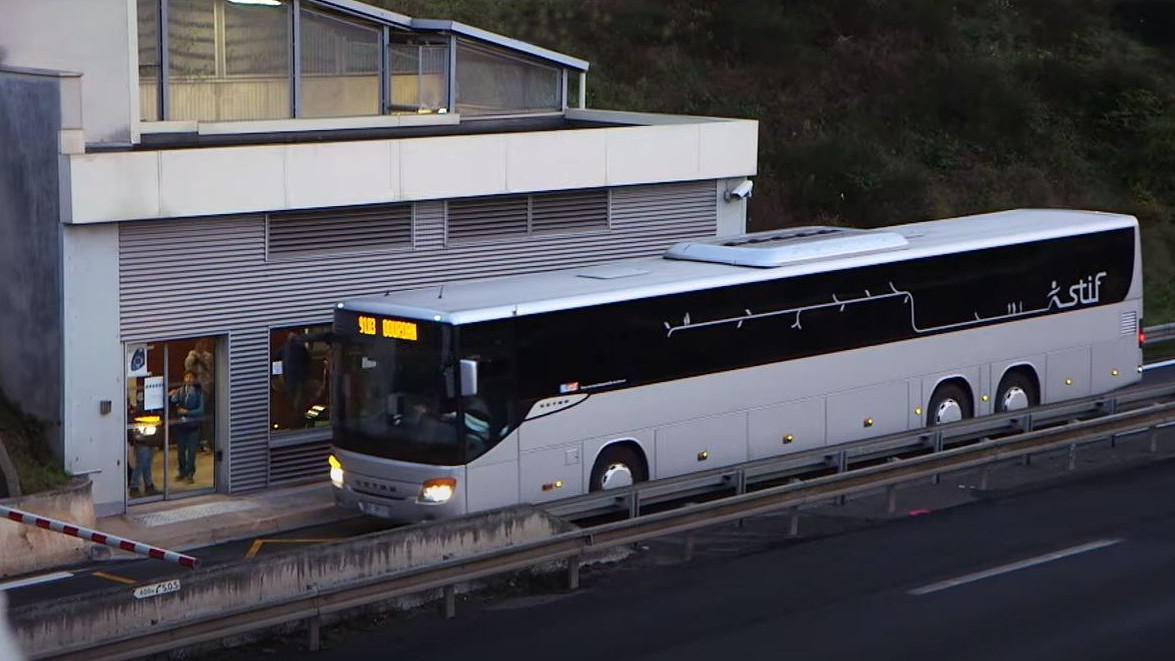
\includegraphics[width=0.7\textwidth]{images/car-express.jpg}
  \caption{Station de car express en Île-de-France : le car ne dévie
    pas de sa voie principale, il emprunte une voie d'arrêt dédiée
    pour l'embarquement et le débarquement des passagers. Sur le plan
    architectural, nul doute que nous pourrions faire preuve d'un peu
    plus d'élégance.}
  \label{fig:car-express}
\end{figure}

Troisièmement, il est primordial de mettre en place des services de
cars express. Contrairement à notre système actuel de cars qui relie
cheminement de village en village, les cars express disposeraient de
stations dédiées sur nos autoroutes et voies rapides, dotées
d'infrastructures sécurisées pour les cyclistes et les piétons, ainsi
que de parkings vélo et voiture afin de ne pas dépendre de la
voiture. Les stations seraient espacées d'environ 5 km les unes des
autres, de manière à ce que chacun qui le souhaite puisse facilement
rejoindre une station de car express en vélo. Les cars ne quitteraient
pas sa route, mais entreraient simplement dans une courte voie de
chargement. De cette manière, les cars express pourraient concurrencer
efficacement les voitures. De tels systèmes peuvent être mis en place
en seulement quelques années, les options ferroviaires suivant là où
le trafic le justifie.

\refs

\textit{Transports : les oubliés de la République: Quand la route reconnecte le territoire}, André Broto, 2022.


\section{De nouvelles gares}

La saturation progressive de la gare de Nantes n’est plus un sujet de
conjecture, mais une réalité à laquelle nous sommes
confrontés. L’importance de la mobilité urbaine exige une réflexion en
profondeur. Ainsi, nous préconisons la création de cinq nouvelles
gares pour désengorger la gare principale et offrir une meilleure
accessibilité.

Malgré les travaux de réaménagement de l'Île de Nantes, ces quartiers
de la ville ne sont pas desservis par d'autres moyens de transport
régional que la voiture individuelle. Il est donc crucial d'adresser
cette insuffisance en intégrant deux nouvelles gares à la ligne
existante et en prolongeant le tronçon restant de la
\href{https://www.mobilitains.fr/tb/t/ligne-johanna-rolland-2021/}{Ligne
  Johanna Rolland} jusqu'au CHU et à l'extrémité de l'île. Cette
extension mènerait à la nouvelle gare des Antilles et comprendrait un
franchissement de la Loire en direction de Chantenay.

\textbf{Médiathèque.} Les travaux du tunnel entre la gare centrale et
Chantenay, très probables dans les dix à vingt prochaines années dus à
l'affaissement lent des caissons dans un sol sableux, est une
opportunité unique. Rétablir la gare de la Bourse en souterrain, et la
mettre en correspondance avec l'arrêt tramway de la Médiathèque,
garantirait une meilleure fluidité des mouvements de passagers en
évitant que tout passager pour Nantes doit changer à la gare centrale.

\textbf{Beaulieu.}
L'extension en cours du centre commercial Beaulieu, d'une superficie
de 5000 mètres carrés, met en évidence l'importance de la mobilité
dans cette zone. Cependant, la création de nouvelles places de
stationnement pour voitures ne répond pas de manière adéquate à cette
exigence. La ligne de TER qui longe cette zone doit être mise à
contribution en créant une gare de Beaulieu, stimulant ainsi la
mobilité durable et minimisant la dépendance à la voiture
individuelle.  Ce serait également le bienvenu pour les commerçants
qui verraient un trafic supplémentaire grâce aux voyageurs en train.

\textbf{Mangin.}
Bien que souvent envisagée en conjonction avec Beaulieu, Mangin a
toutes les raisons d'avoir sa propre station. La distance entre
Beaulieu et Mangin, supérieure à un kilomètre, justifie cette
distinction. D’ailleurs, tous les trains n'ont pas besoin de s'arrêter
dans ces deux gares, même si la fréquence actuelle des trains rend
difficilement imaginable une alternance. Les exemples, comme celui du
RER C à Paris, réfutent l'idée selon laquelle deux gares ne peuvent
coexister à une distance de marche de 15 minutes.

\textbf{CHU.}  Le nouveau CHU, générateur de presque 20,000 emplois,
et attirant chaque jour de nombreux patients et visiteurs sans parler
de ceux qui se déplacent pour les écoles, entreprises et commerces qui
ouvrent dans son ombre, nécessite une liaison ferroviaire
régionale. L'espace permettant une desserte depuis le nord et le sud
est toujours disponible. Si le tramway en cours de construction est
une avancée pour les Nantais, il ne répond pas entièrement aux besoins
de ceux venant de régions éloignées, qui pourraient ainsi délaisser
leur voiture.

\textbf{La gare des Antilles et son pont.}  Desservir l’extrémité de
l'Île de Nantes renforcera la cohérence du réseau. Un franchissement
de la Loire (le pont des Antilles, proposé) pour rejoindre la gare de
Chantenay et les lignes en direction de Saint Nazaire, Le Croisic,
Redon, et la Bretagne, est un levier stratégique. Cela allègerait
considérablement la sollicitation de la gare centrale de Nantes,
évitant que tous les trains y transitent.  De plus, en cas de travaux
ou d'incident dans le tunnel entre Chantenay et la gare centrale de
Nantes, une telle alternative préserverait la connectivité entre
Nantes, l'ouest et le nord.

% https://www.20minutes.fr/nantes/3181159-20211124-nantes-centre-commercial-beaulieu-etend-recevoir-primark

% https://actu.fr/pays-de-la-loire/nantes_44109/nantes-pourquoi-y-a-t-il-des-travaux-pres-du-centre-commercial-beaulieu_41278110.html


\section{La gare centrale de Nantes}

La gare centrale de Nantes, point névralgique du réseau ferroviaire de
la région Pays de la Loire, connaît une affluence sans précédent
récent. Cette croissance reflète la vitalité de la région, mais elle
pose également un ensemble de défis majeurs en termes d'aménagement,
de logistique et de mobilité.

La première réponse à cette affluence est d'assurer une circulation
fluide et sécurisée des voyageurs. Pour ce faire, il est impératif de
penser à l'espace autrement. La mise en place d'un passage surélevé à
l'extrémité est des quais est une solution viable. Ce passage
faciliterait non seulement le flux de voyageurs entre les différentes
voies, mais créerait également un lien direct avec la station de
tramway de Manufacture au nord et avec le nouveau quartier d'Europe au
sud.

En reliant la gare au quartier d'Europe et à la station de tramway
(sans construction de parking voiture supplémentaire), nous
permettrons aux voyageurs d'accéder facilement à la gare depuis
différentes parties de la ville. Cette connectivité améliorée
favoriserait une transition fluide entre les différents modes de
transport, contribuant ainsi à réduire la congestion routière et les
émissions de carbone.

Une deuxième réponse et enjeu majeur concerne la logistique des trains
eux-mêmes. La gare centrale ne doit plus être considérée uniquement
comme un point de terminaison pour tous les trains. En effet, une
grande partie des trains régionaux pourrait continuer leur trajet vers
une autre destination. Même les trains longue distance pourraient
continuer leur trajet au moins jusqu'à Chantenay. Cette continuité
présente plusieurs avantages : elle fluidifie le trafic, évite les
engorgements dans les voies de garage et permet une meilleure gestion
de l'espace ferroviaire.


\section{L'accès pédestre et cycliste aux transports collectifs}

Pour parvenir à une augmentation de la fréquence et de l'amplitude du
service de transport public, il est primordial d'accroître l'accès à
ces services. Aujourd'hui, une grande partie de la population accède
aux services de transport en commun en voiture. Cette pratique n'est
ni durable ni écologiquement souhaitable.

Un des principaux obstacles est l'accès aux transports publics à pied
ou à vélo. Face à ce défi, il est impératif de garantir que chaque
arrêt de bus, tramway, et car ainsi que toute gare ferroviaire soit
accessible en toute sécurité en dix minutes à pied (soit une distance
d'environ 500 mètres) et à vélo (soit une distance d'environ 3 km).

Cependant, assurer une bonne accessibilité n'est qu'une partie de la
solution. Il est également essentiel de fournir des installations de
stationnement adaptées pour les vélos. Le caractère "adéquat" de ces
installations peut varier selon la localité. Dans les zones urbaines,
où les contraintes sont plus marquées en raison de la densité et des
risques de vol, le besoin en matière de sécurité et de protection
contre les intempéries est plus élevé.

À l'inverse, dans les zones rurales, les exigences sont souvent moins
strictes. Une simple attache ou appui, éventuellement couverte d'un
toit pour le protéger de la pluie, suffirait généralement.


\section{Harmonisation du matériel roulant}

La région de Nantes, avec son dynamisme économique et démographique,
mérite une attention toute particulière en ce qui concerne sa
mobilité. Deux des lignes majeures, Nantes-Clisson (inaugurée en tant
que tram-train le 15 juin 2011) et Nantes-Châteaubriant (ouverte le 24
février 2014), ont adopté du matériel roulant spécifique, différent du
reste du système ferroviaire français. Cette décision, quoique basée
sur des raisons politiques, économiques, et contextuelles, a des
répercussions significatives sur la mobilité de la région.

\begin{figure}[ht]
  \centering
  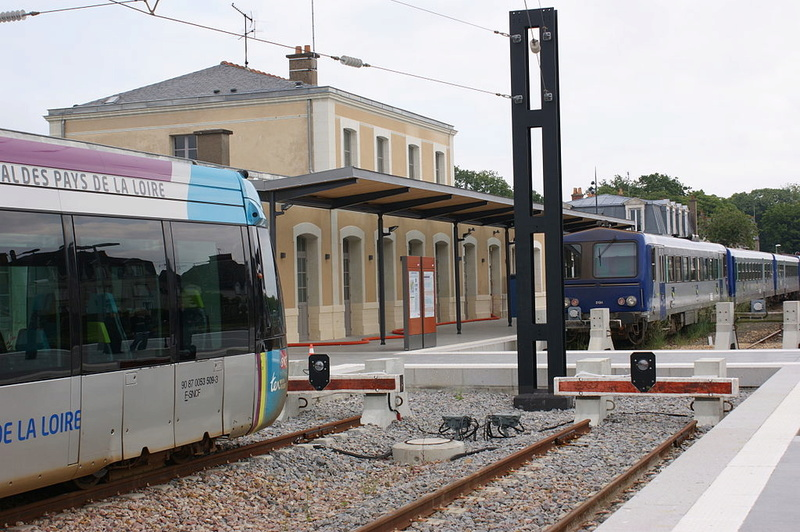
\includegraphics[width=0.7\textwidth]{images/gare-chateaubriant-1.jpg}
  \caption{À la gare de Châteaubriant, divers matériels roulants
    présentent des besoins électriques et de signalisation
    incompatibles, compromettant la liaison entre les régions de
    Nantes et Rennes.}
  \label{fig:chateaubriant}
\end{figure}

Actuellement, la SNCF, ou son futur concessionnaire (également la
SNCF), se trouve dans l'obligation de gérer l'exploitation,
l'entretien et la maintenance de deux systèmes distincts, doublant
ainsi les efforts en termes de ressources humaines et
financières. Cette hétérogénéité du matériel roulant empêche une
fluidité opérationnelle. Par exemple, une liaison directe entre Nantes
et Rennes via Châteaubriant est entravée à cause de l'incompatibilité
technique (voir figure~\ref{fig:chateaubriant}). Les gares intermédiaires
subissent également cette décision, ne permettant pas aux TER
traditionnels de s'arrêter, comme c'est le cas à Savenay.

De surcroît, les infrastructures actuelles, notamment la hauteur des
quais, ne sont pas adaptées aux TER traditionnels. C'est la raison
pour laquelle les tram-trains de Clisson stationnent en périphérie de
la gare de Nantes (voir figure~\ref{fig:clisson}) et que des travaux
d'ajustement ont dû être réalisés sur les quais de la ligne
Nantes-Clisson.

\begin{figure}[ht]
  \centering
  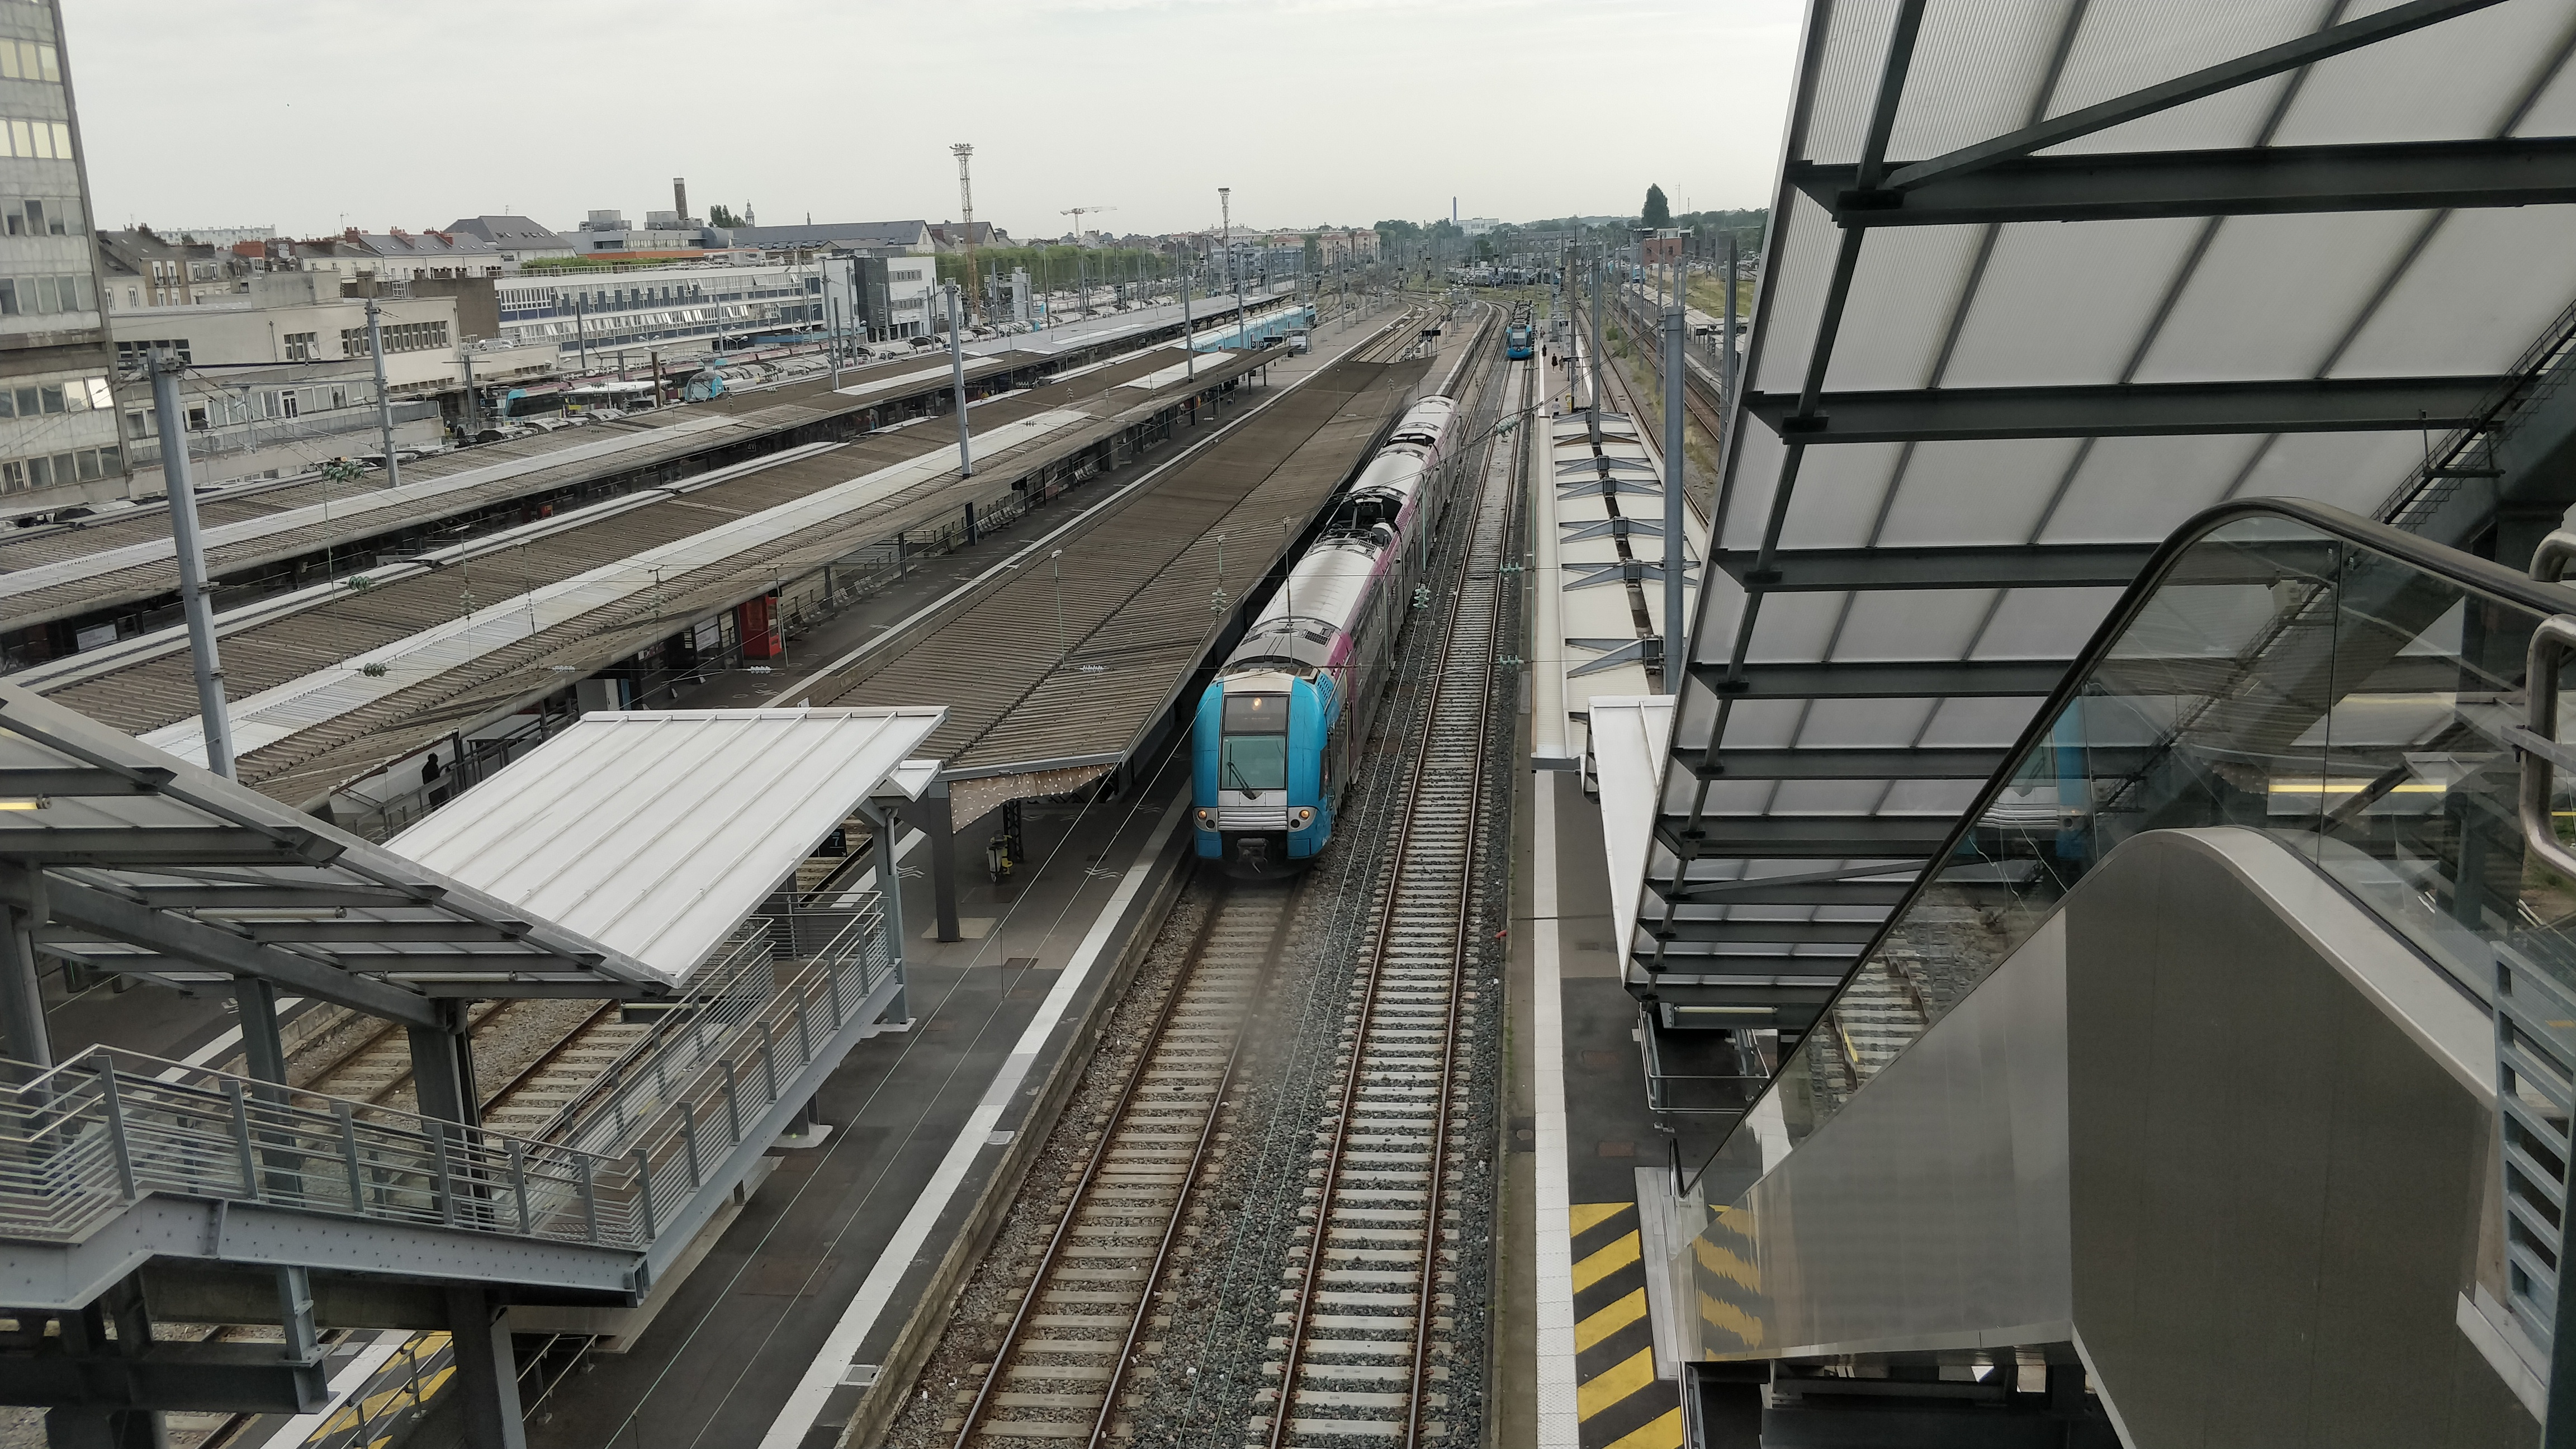
\includegraphics[width=0.7\textwidth]{images/IMG_20230908_104847-clisson.jpg}
  \caption{En premier plan sur la voie de gauche : un TER
    traditionnel.  À l'arrière-plan sur la voie de droite, bien plus
    éloigné et à peine visible, le train-tram en direction de Clisson.
    Si combiner le train et la marche représente une forme de
    multimodalité, ce n'est pas nécessairement la vision typique que
    l'on en a.}
  \label{fig:clisson}
\end{figure}

Concernant les vitesses, il est à noter que les tram-trains ne
dépassent pas 100 km/h, et cette vitesse est encore plus réduite à 30
km/h en zone métropolitaine entre Nantes et
La~Chapelle-sur-Erdre. Ainsi, ils ne peuvent rivaliser avec les
véhicules personnels en termes de rapidité, rendant le choix du train
moins attractif pour beaucoup de trajets.

Le matériel roulant sur ces deux lignes approche les 15 ans depuis son
acquisition par la région (commandé le 25 avril 2007) avec 12 ans en
exploitation. Il est crédible de parler de son renouvellement pour
2050.

Devant ces constats, la nécessité d'harmoniser le matériel roulant
devient impérative pour optimiser l'exploitation ferroviaire. Une
telle démarche permettrait une meilleure desserte pour les habitants
de Nantes et de la région Pays de la Loire, tout en rationalisant les
coûts d'exploitation et de maintenance.

\refs

\begin{itemize}
\item L’échec très discret du tram‐train Nantes‐Châteaubriant\\
\link{https://www.mediacites.fr/enquete/nantes/2017/09/20/lechec-tres-discret-du-tram-train-nantes-chateaubriant/}
\item TRIBUNE – Un avenir pour la ligne Rennes‐Châteaubriant‐Nantes\\
\link{https://www.mediacites.fr/forum/nantes/2017/09/21/un-avenir-pour-la-ligne-rennes-chateaubriant-nantes/}
\item Tram‐train Nantes‐Châteaubriant : quand la Région s’en prend à \dots la Région\\
\link{https://www.mediacites.fr/complement-denquete/nantes/2017/12/07/tram-train-nantes-chateaubriant\%e2\%80\%af-quand-la-region-sen-prend-a-la-region/}
\item Nantes‐Châteaubriant : l’avenir de plus en plus incertain du tram‐train
\link{https://www.mediacites.fr/complement-denquete/nantes/2018/11/15/nantes-chateaubriant-lavenir-de-plus-en-plus-incertain-du-tram-train/}
\item Le tram‐train Nantes – Châteaubriant patine toujours
\link{https://www.mediacites.fr/breve/nantes/2021/01/07/le-tram-train-nantes-chateaubriant-patine-toujours/}
\item Tram‐train Nantes‐Châteaubriant : (encore) 1,5 million d’euros de travaux avant l’ouverture à la concurrence
\link{https://www.mediacites.fr/breve/nantes/2021/12/16/tram-train-nantes-chateaubriant-encore-15-million-deuros-de-travaux-avant-louverture-a-la-concurrence/}
\end{itemize}


\section{Intégration fluide du vélo, train et car}

Le vélo, plus qu'une simple activité sportive, est devenu un élément
central de la mobilité contemporaine. Dans ce contexte, il est crucial
de repenser nos services TER et de transport par car pour qu'ils
répondent aux besoins diversifiés des cyclistes, reflétant par la même
occasion les évolutions sociétales en matière de déplacement.

\begin{figure}[ht]
  \centering
  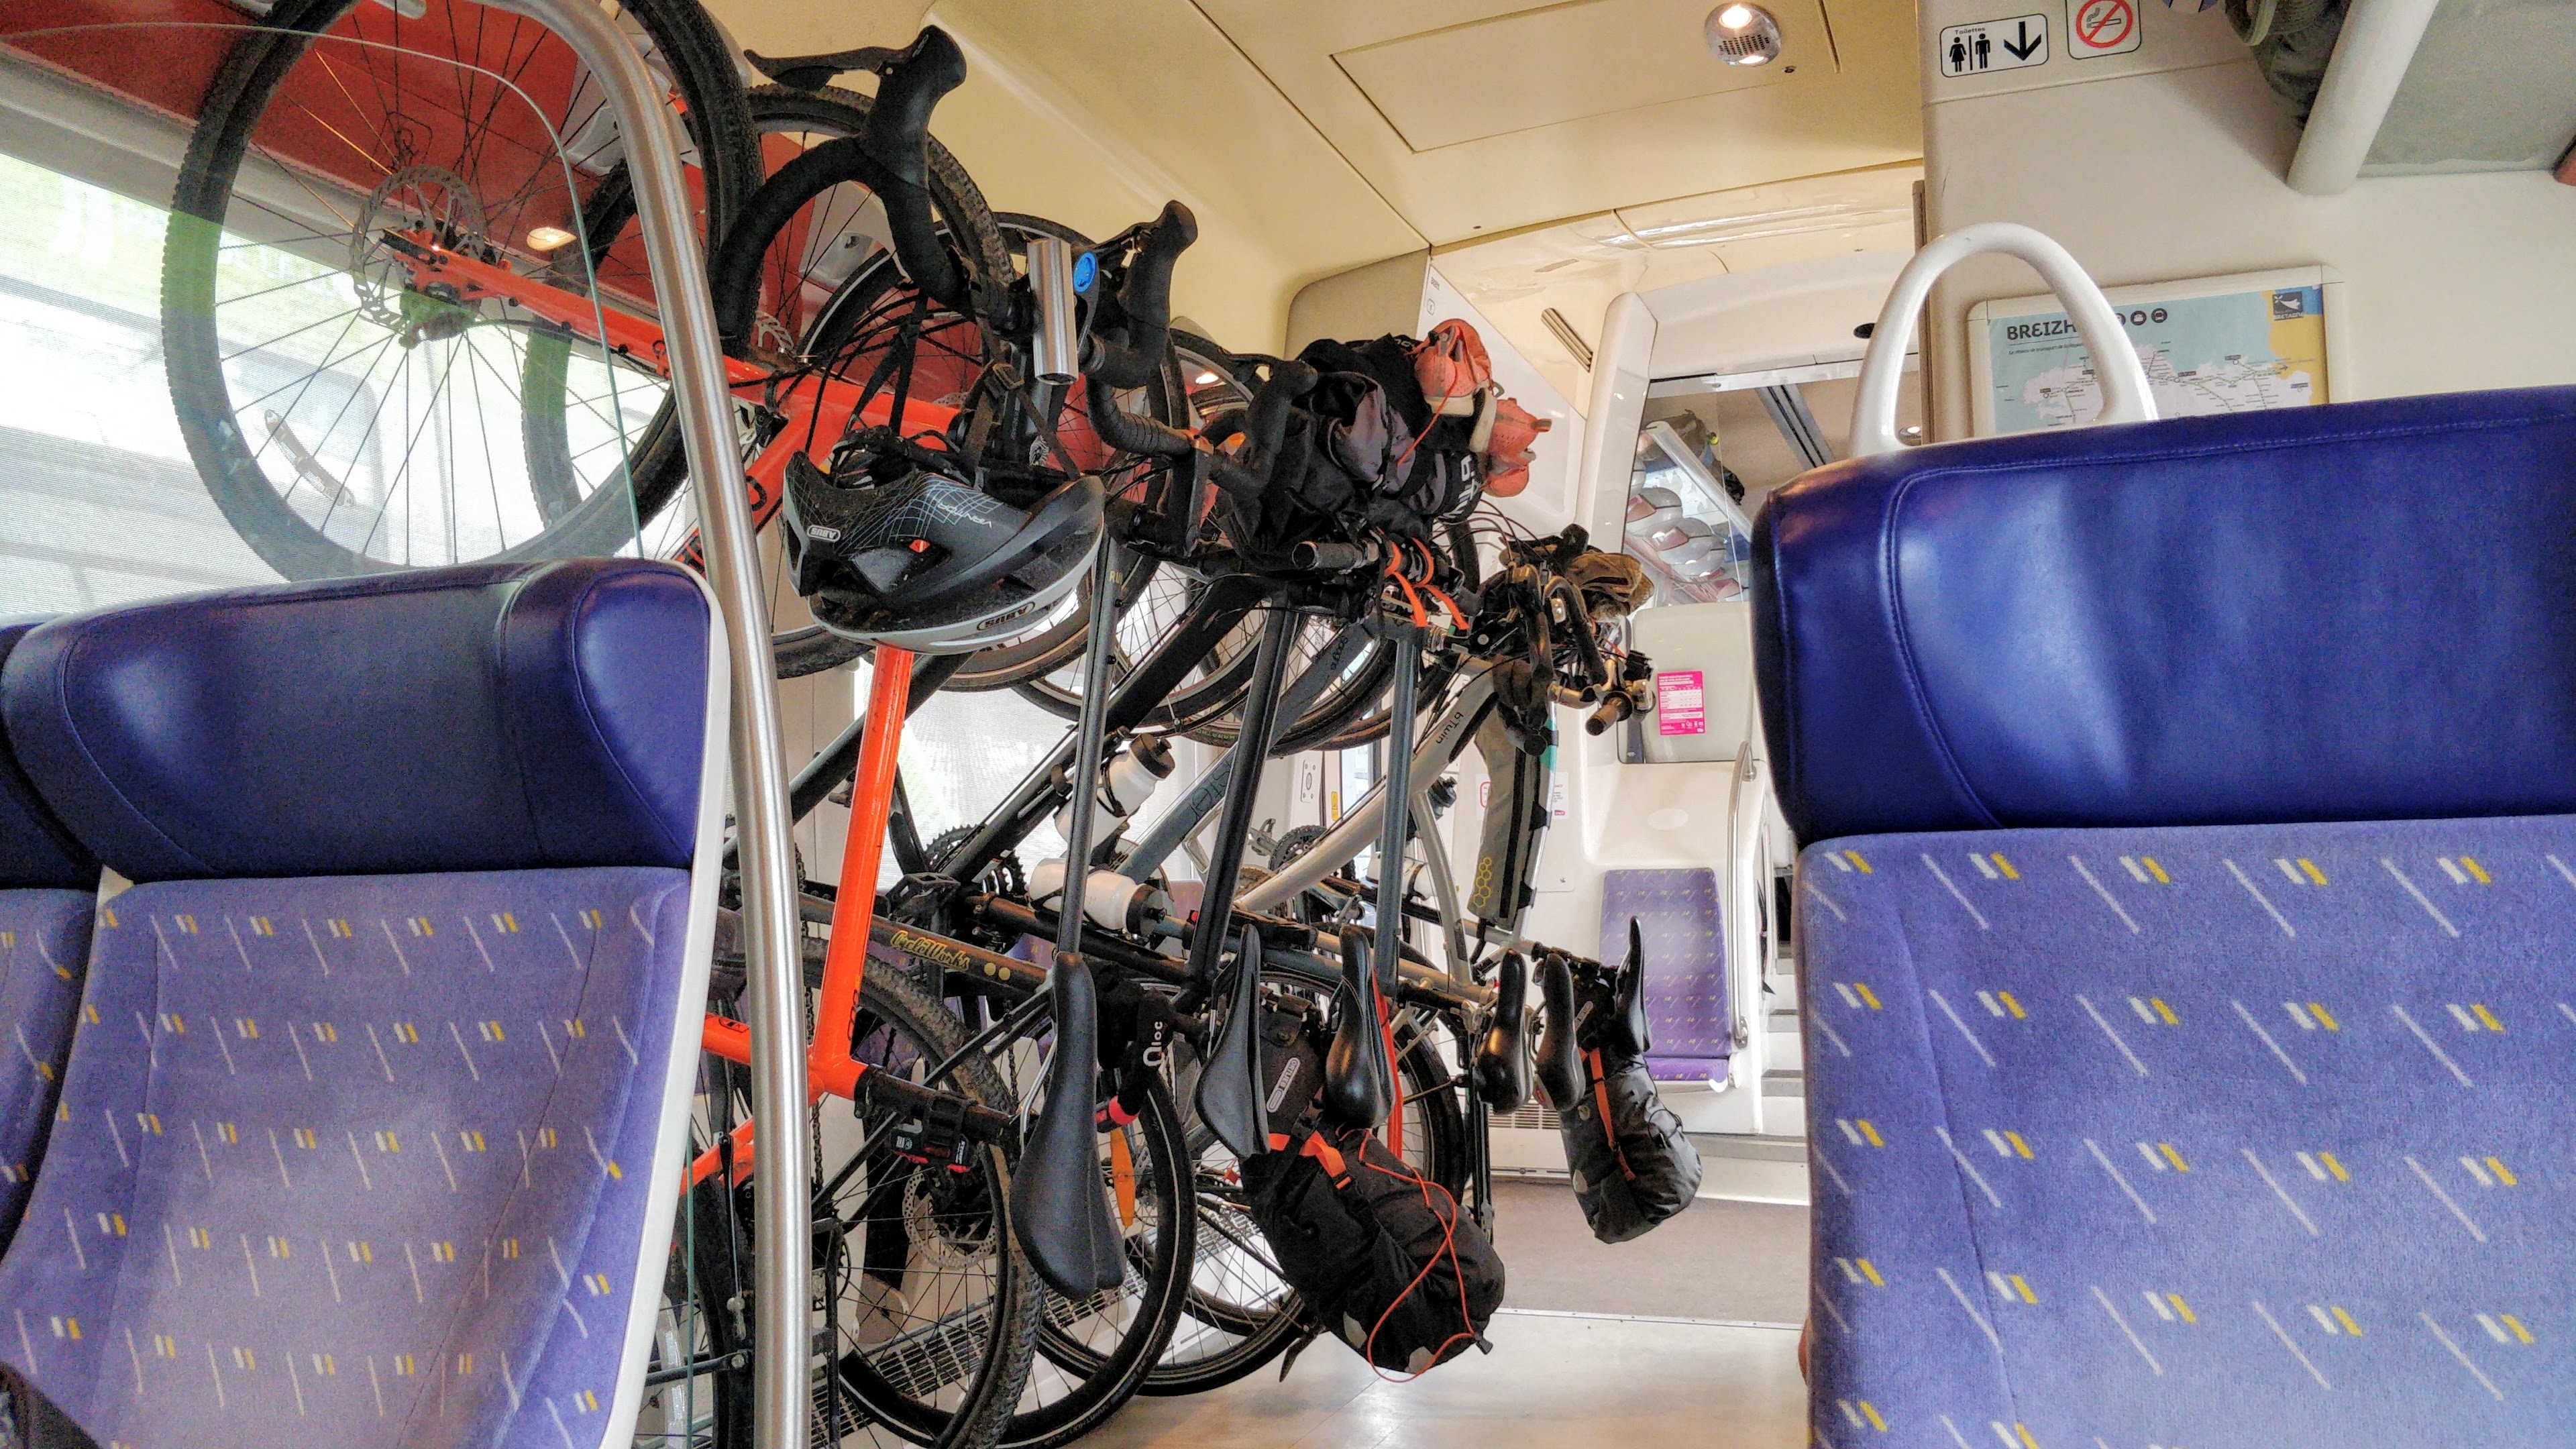
\includegraphics[width=0.7\textwidth]{images/IMG-20220729-WA0001-TER-hanging.jpeg}
  \caption{Cessons de préconiser le rangement vertical des vélos :
    cette idée découle d'une perception naïve où tous les cyclistes
    sont sportifs dotés de vélos légers. Dans un monde visant à
    optimiser la mobilité, nombreux sont les cyclistes qui sont
    jeunes, âgés, ou n'ont pas autant de force physique, et utilisent
    des vélos à assistance électrique ou équipés de sacoches.  De
    plus, ranger un vélo horizontalement facilite la montée et la
    descente des trains, contrairement au rangement vertical.}
  \label{fig:train-velo-vertical}
\end{figure}

Aujourd'hui, la bicyclette n'est plus cantonnée à une utilisation
sportive ou récréative. Elle est un outil quotidien pour de nombreux
citoyens, indépendamment de leur âge, pour leurs déplacements
professionnels ou personnels. Pourtant, nos TER semblent encore pensés
pour des cyclistes sportifs avec vélos légers et sans bagages (voir
figure~\ref{fig:train-velo-vertical}). Quant à nos cars,
l'embarquement de vélos y est souvent complexe, voire inexistant. Une
telle vision ne capture pas l'essence de la mobilité actuelle.

Il est donc urgent d'entamer une transformation radicale de nos TER et
de notre service de cars pour intégrer de manière efficace et pratique
les vélos. Imaginons un système de rangement horizontal (voir
figure~\ref{fig:train-velo-francais-horizontal}), ``roll-on,
roll-off'', où l'on pourrait monter et descendre aisément avec son
vélo, qu'il soit traditionnel ou à assistance électrique, avec ou sans
bagages.

\begin{figure}[ht]
  \centering
  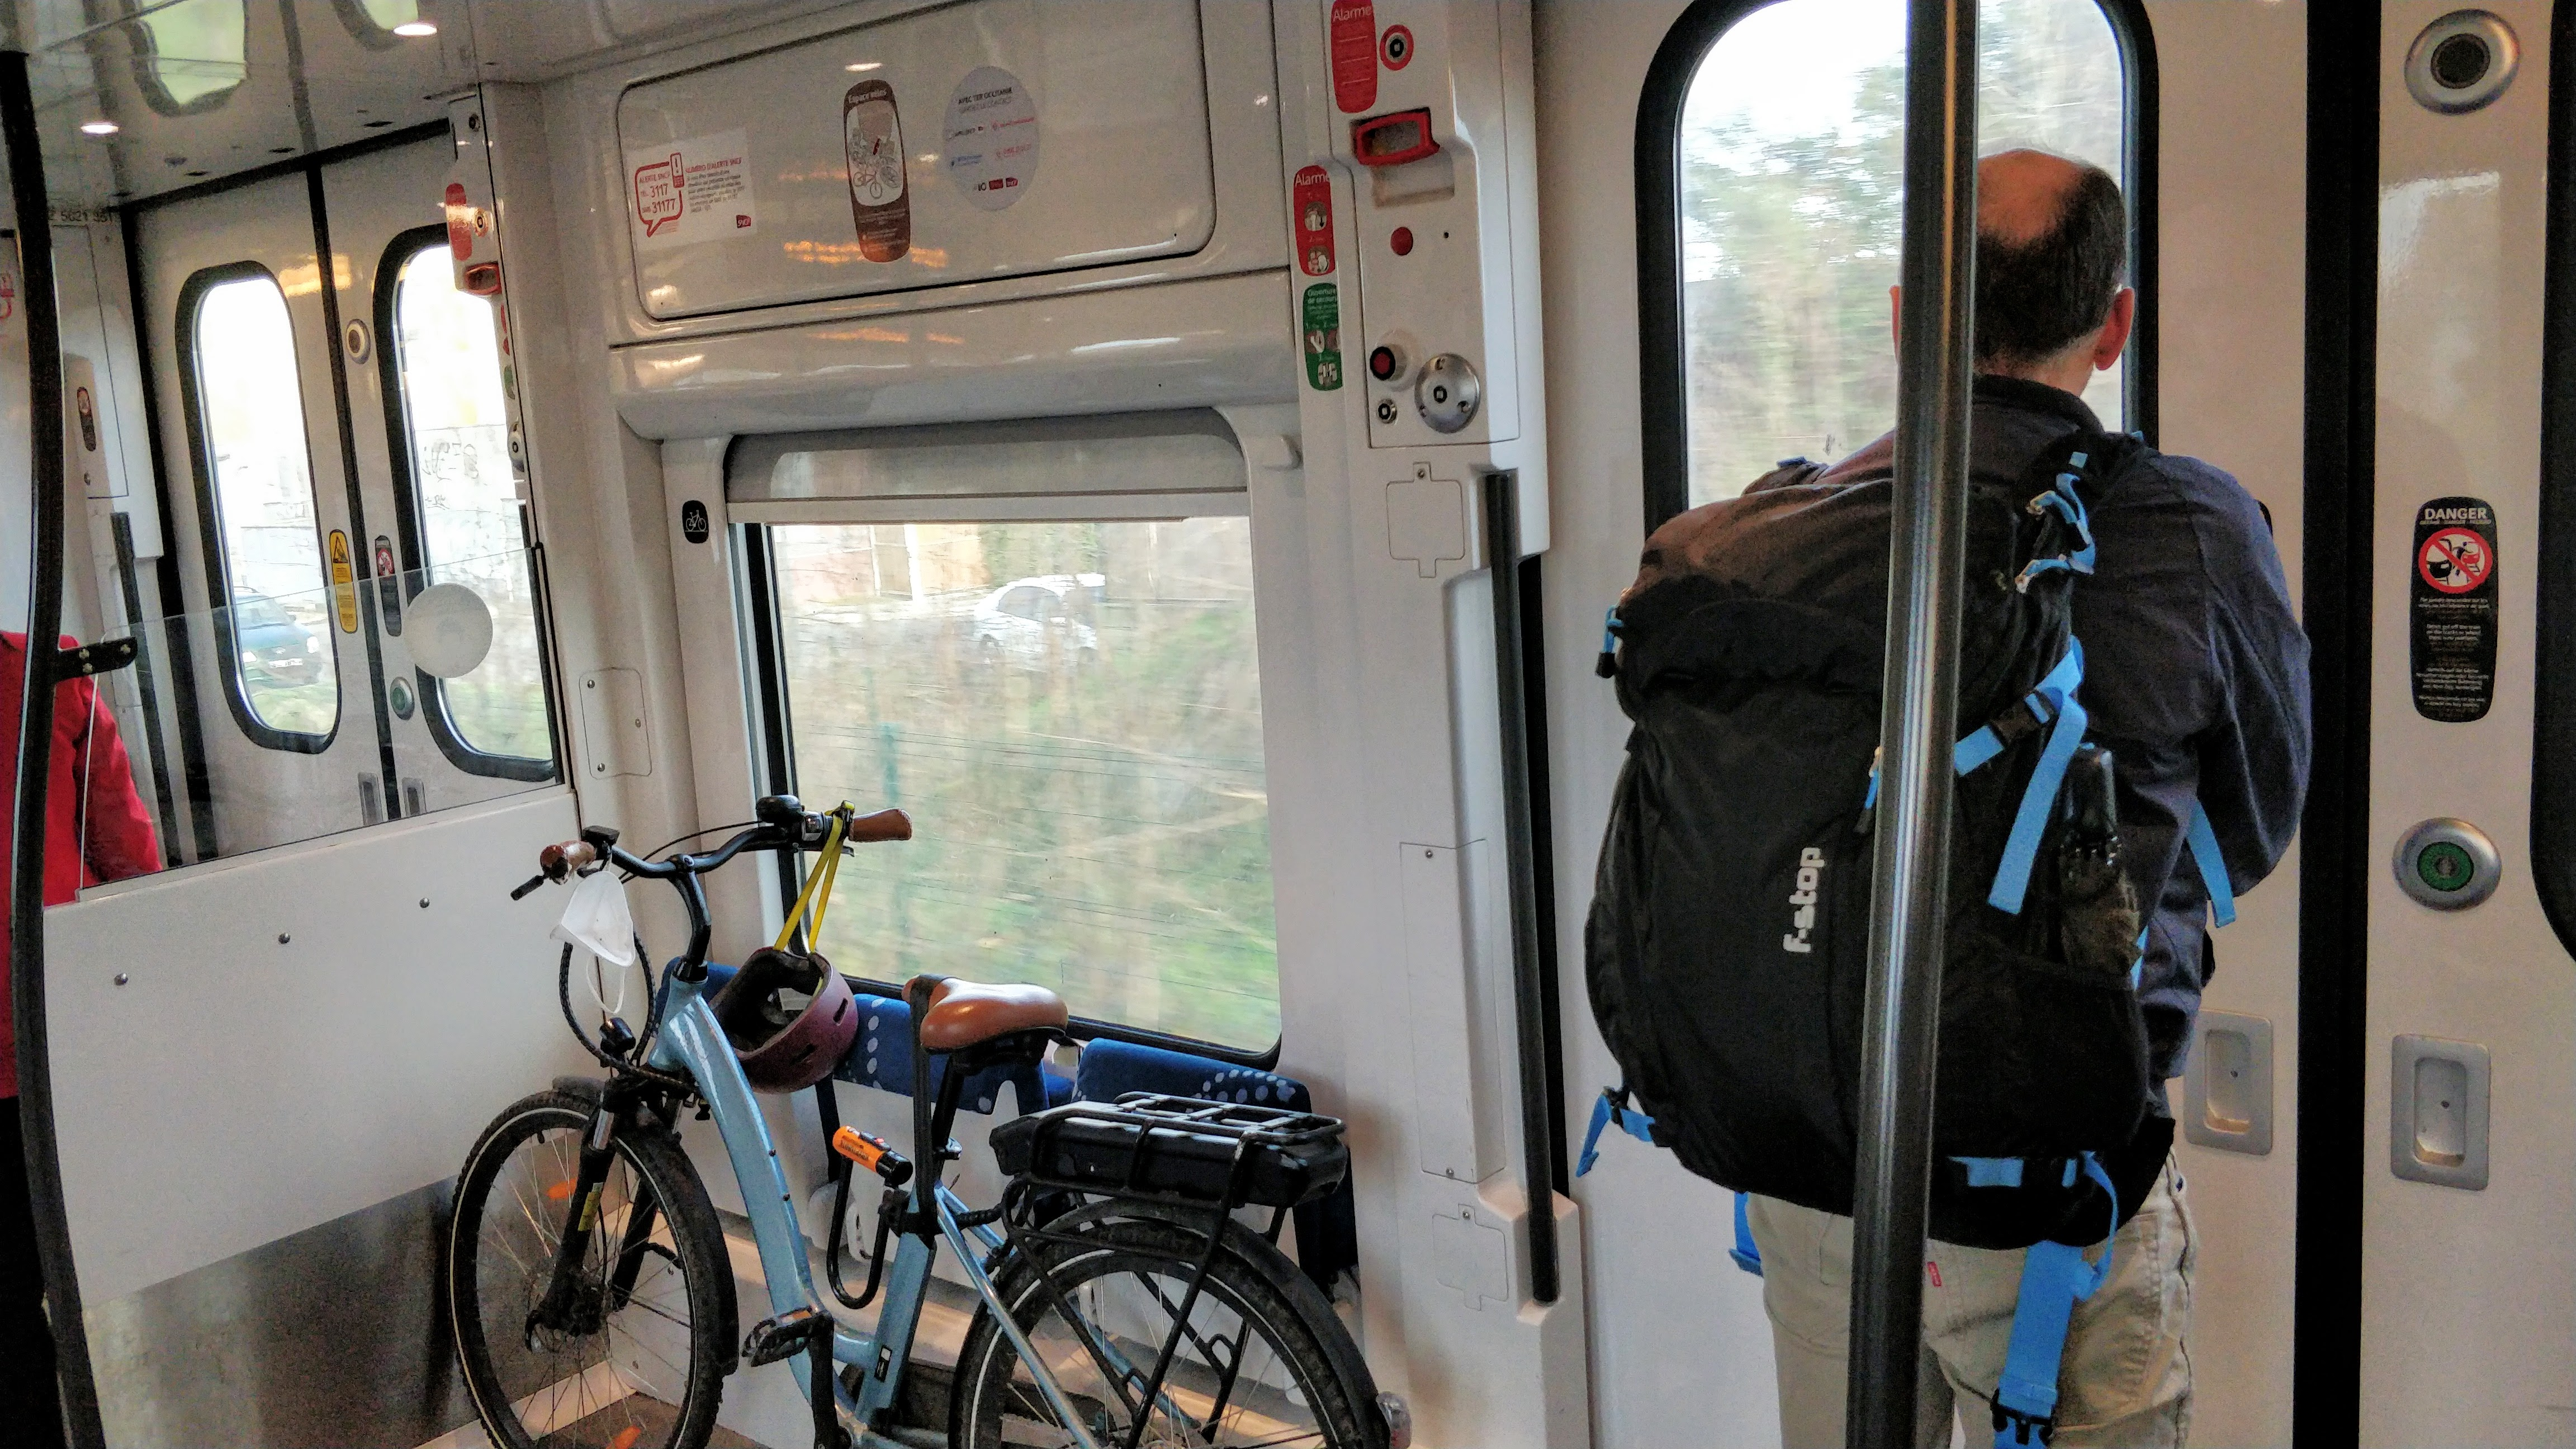
\includegraphics[width=0.7\textwidth]{images/IMG_20221223_145849-TER-horizontal.jpg}
  \caption{Des sièges pliants et polyvalents à bord d'un train
    français avec vélo rangé en horizontal.  Cet espace vélo suffit
    pour trois vélos.}
  \label{fig:train-velo-francais-horizontal}
\end{figure}

\begin{figure}[ht]
  \centering
  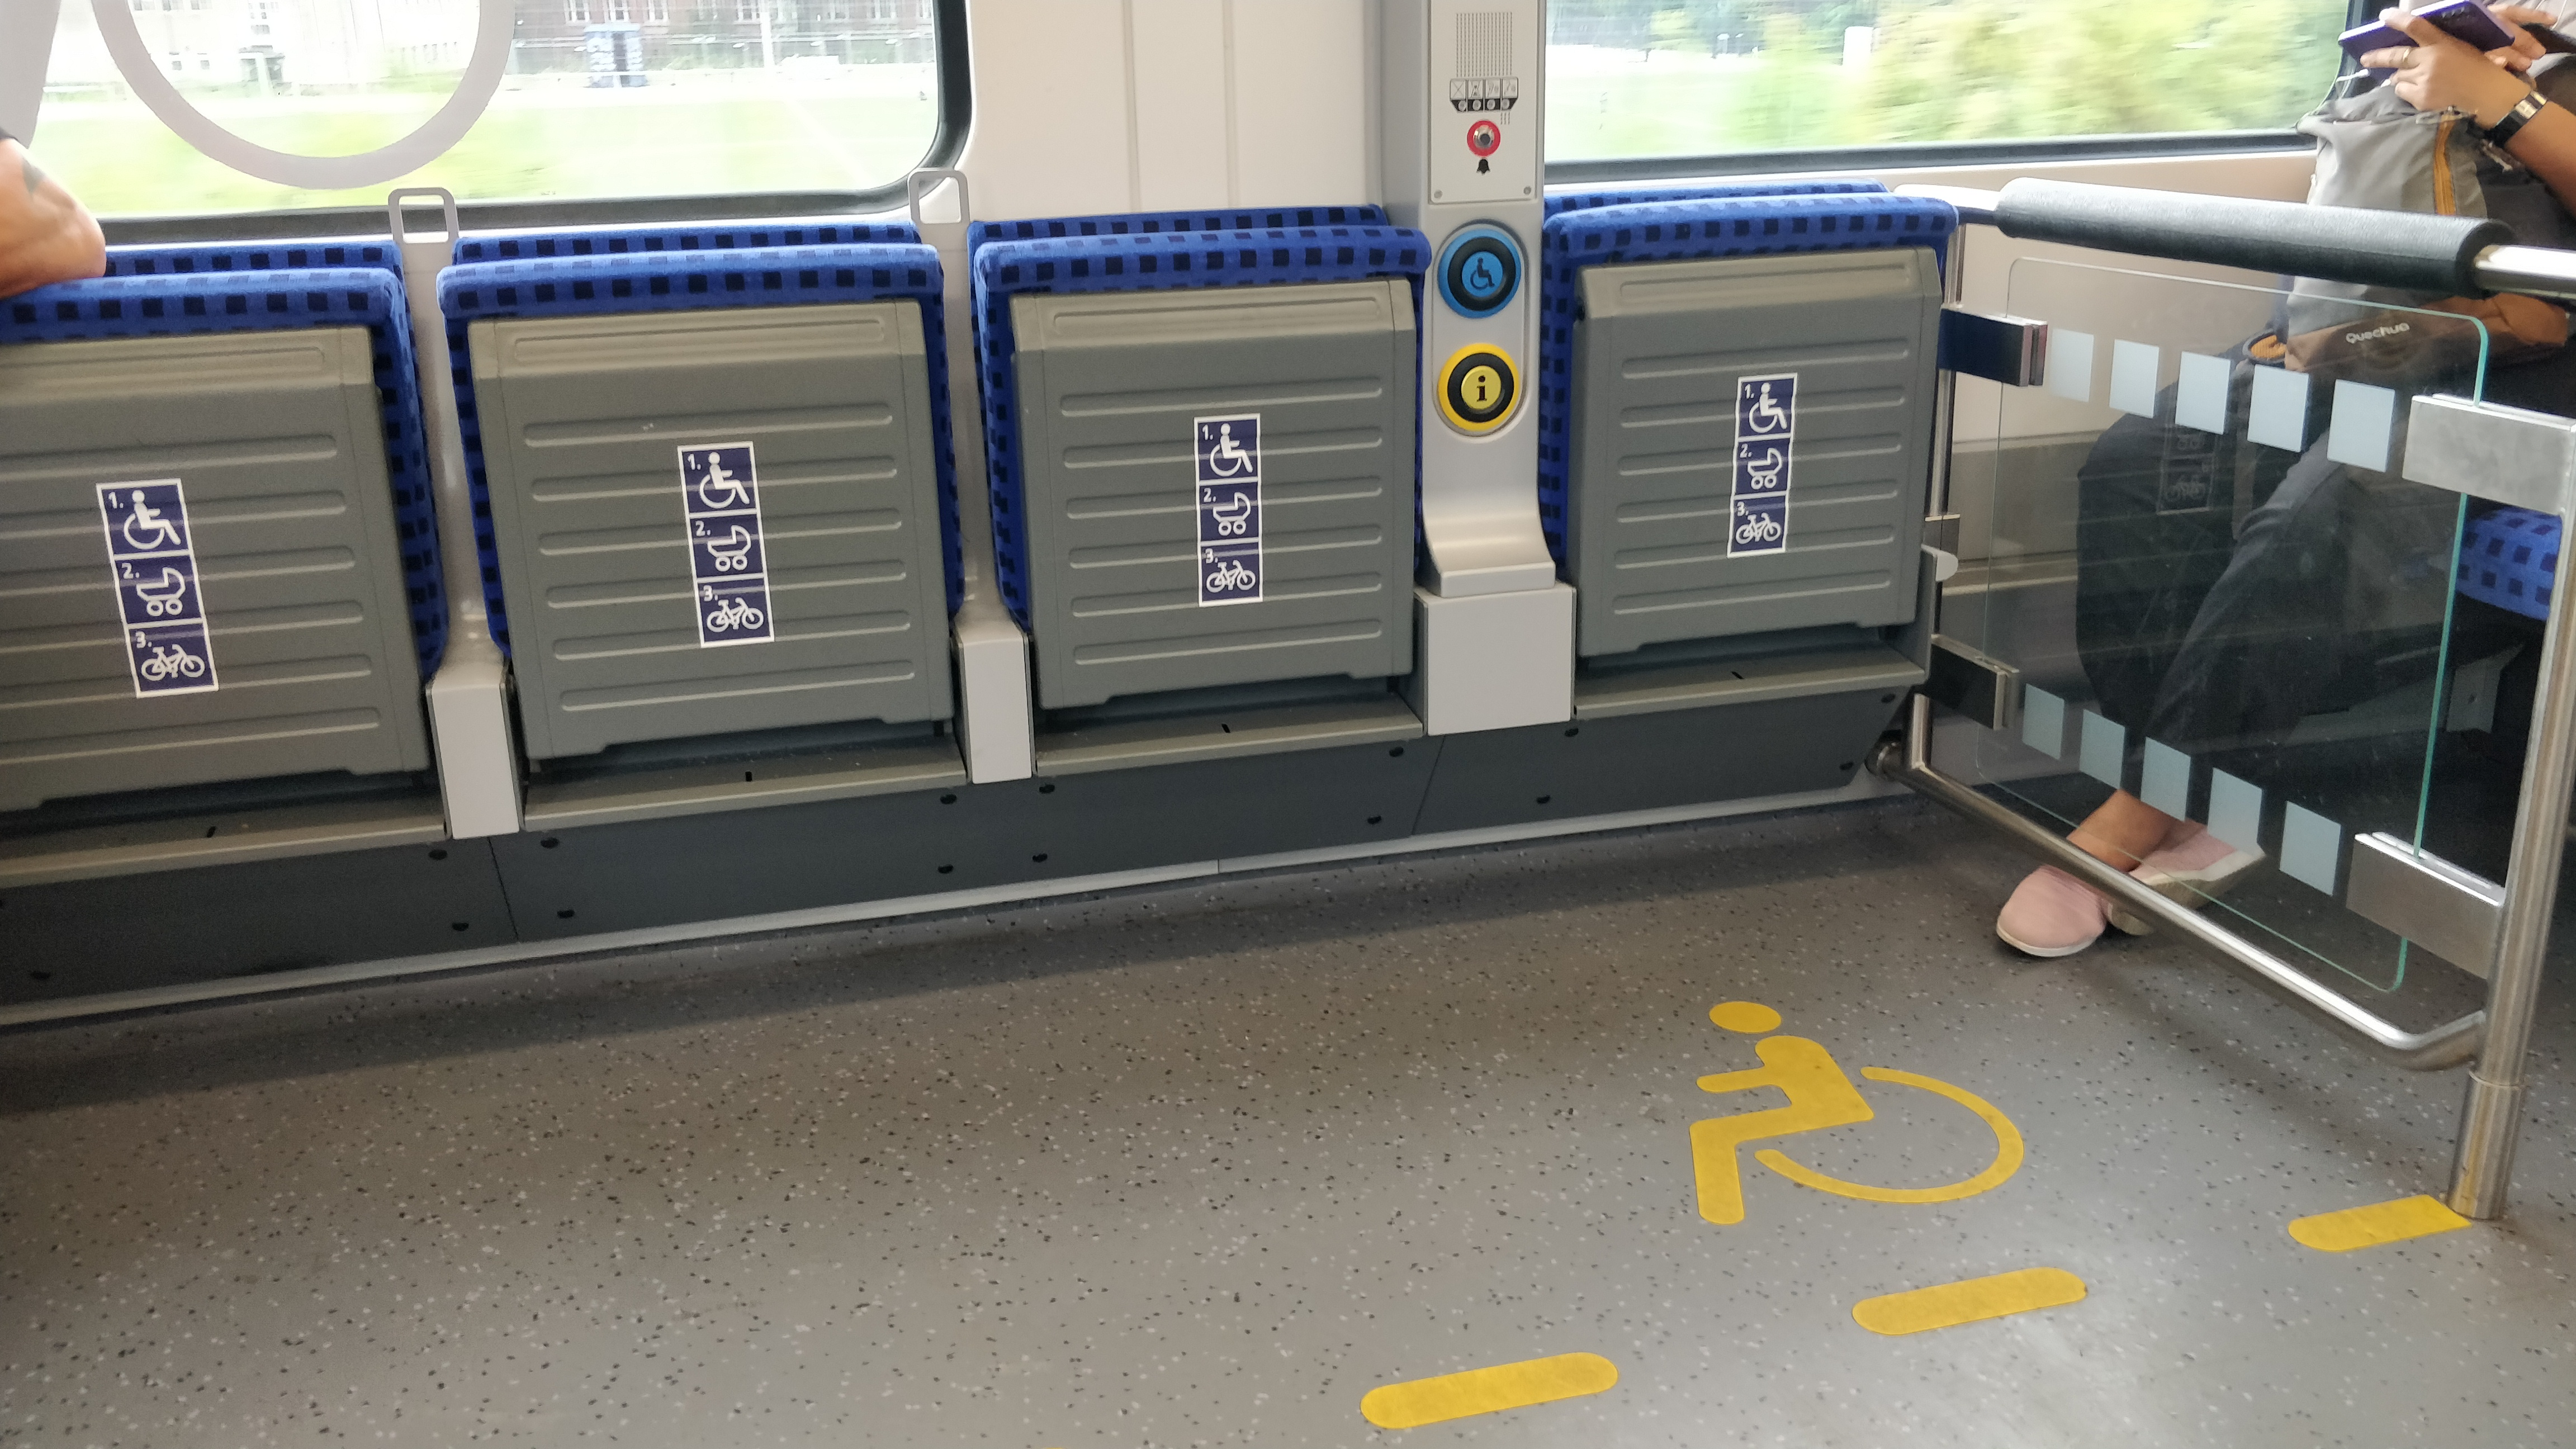
\includegraphics[width=0.7\textwidth]{images/IMG_20230826_102932-seats.jpg}
  \caption{Des sièges pliants et polyvalents à bord d'un train
    allemand, avec des indications de priorité pour les PMR, les mères
    avec jeunes enfants et les vélos.  Rien ne nous empêche de
    proposer la même chose en car.}
  \label{fig:train-velo-allemand-horizontal}
\end{figure}

Les espaces dédiés à ces vélos devraient être polyvalents (voir
figure~\ref{fig:train-velo-allemand-horizontal}) : des sièges pliants
permettraient, par exemple, de favoriser aussi bien les cyclistes que
les personnes à mobilité réduite, les femmes enceintes et l'ensemble
des usagers.

En adaptant nos TER et nos cars à la réalité multifacette du vélo
comme élément clé de la mobilité et en promouvant une intégration
harmonieuse entre le vélo et le train et car, avec accès sans barrière
et rangement horizontal, nous jetons les bases d'un système de
transport innovant et inclusif pour le futur.
